\documentclass[11pt]{report}
\usepackage[utf8]{inputenc}
\usepackage[danish]{babel}
\usepackage [T1]{fontenc}
\usepackage[margin=2.5cm]{geometry}
\usepackage[hidelinks]{hyperref}
\usepackage{graphicx}
\graphicspath{{figures/}{Billeder/}}
\usepackage{listings}
\usepackage{color}
\usepackage{adjustbox}
\usepackage{tocloft}
\usepackage{listings}
\usepackage{enumitem}

\setlength{\parskip}{12pt}

\definecolor{dkgreen}{rgb}{0,0.6,0}
\definecolor{gray}{rgb}{0.5,0.5,0.5}
\definecolor{mauve}{rgb}{0.58,0,0.82}

\lstset{frame=tb,
  language=Java,
  aboveskip=3mm,
  belowskip=3mm,
  showstringspaces=false,
  columns=flexible,
  basicstyle={\small\ttfamily},
  numbers=none,
  numberstyle=\tiny\color{gray},
  keywordstyle=\color{blue},
  commentstyle=\color{dkgreen},
  stringstyle=\color{mauve},
  breaklines=true,
  breakatwhitespace=true,
  tabsize=3
}



\definecolor{bluekeywords}{rgb}{0.13,0.13,1}
\definecolor{greencomments}{rgb}{0,0.5,0}
\definecolor{turqusnumbers}{rgb}{0.17,0.57,0.69}
\definecolor{redstrings}{rgb}{0.5,0,0}

\lstdefinelanguage{FSharp}
                {morekeywords={let, new, match, with, rec, open, module, namespace, type, of, member, and, for, in, do, begin, end, fun, function, try, mutable, if, then, else},
    keywordstyle=\color{bluekeywords},
    sensitive=false,
    morecomment=[l][\color{greencomments}]{///},
    morecomment=[l][\color{greencomments}]{//},
    morecomment=[s][\color{greencomments}]{{(*}{*)}},
    morestring=[b]",
    stringstyle=\color{redstrings}
    }
\usepackage{amsmath}
\title{Systemudvikling Eksamen}


\author{
  Martin, Frederiksen\\
  \texttt{cph-mf237@cphbusiness.dk}\\
  A klassen
  \and
  Andreas, Vikke\\
  \texttt{cph-av105@cphbusiness.dk}\\
  A klassen
  \and
  Asger, Sørensen\\
  \texttt{cph-as466@cphbusiness.dk}\\
  A klassen
  \and
  William, Huusfeldt\\
  \texttt{cph-wh106@cphbusiness.dk}\\
  A klassen
  \and
  Emil, Svensmark\\
  \texttt{cph-eb112@cphbusiness.dk}\\
  A klassen
}

\date{}

\begin{document}
\maketitle

\renewcommand{\cftchapleader}{\cftdotfill{\cftdotsep}}
\tableofcontents
\newpage

\chapter*{1. Indledning}
\addcontentsline{toc}{chapter}{1. Indledning}

\chapter*{2. Systemudviklingsmodel og metode}
\addcontentsline{toc}{chapter}{2. Systemudviklingsmodel og metode}
\section*{2.2. Virksomhedens krav}
\addcontentsline{toc}{section}{2.2. Virksomhedens krav}
\section*{2.3. Virksomhedens vision}
\addcontentsline{toc}{section}{2.3. Virksomhedens vision}

\chapter*{3. Use Case Diagram}
\addcontentsline{toc}{chapter}{3. Use Case Diagram}

\chapter*{4. 1 udvalgt Use Case}
\addcontentsline{toc}{chapter}{4. 1 udvalgt Use Case}

\chapter*{5. Outsorcing proces}
\addcontentsline{toc}{chapter}{5. Outsorcing proces}

\chapter*{6. Scrum plan}
\addcontentsline{toc}{chapter}{6. Scrum plan}

\chapter*{7. XP plan}
\addcontentsline{toc}{chapter}{7. XP plan}

\chapter*{8. Scrum-proces}
\addcontentsline{toc}{chapter}{8. Scrum-proces}
\section*{8.1. Roles}
\addcontentsline{toc}{section}{8.1. Roles}
\section*{8.1. Ceremonies}
\addcontentsline{toc}{section}{8.1. Ceremonies}
\section*{8.1. Artifacts}
\addcontentsline{toc}{section}{8.1. Artifacts}


\chapter*{9. XP-proces}
\addcontentsline{toc}{chapter}{9. XP-proces}


\chapter*{10. Reflektion over processen}
\addcontentsline{toc}{chapter}{10. Reflektion over processen}


\chapter*{11. Bilag}
\addcontentsline{toc}{chapter}{11. Bilag}

\section*{11.1 Bilag 1) Fully dressed use case}
\addcontentsline{toc}{section}{11.1 Bilag 1) Fully dressed use case }
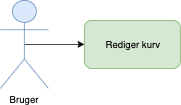
\includegraphics[width=8cm, height=5cm]{FullyDressedUseCase.png}

\noindent \textbf{Use case:} rediger kurv

\noindent \textbf{Primary Actor:} Bruger

\noindent \textbf{Goal:} At redigere produkter i brugerens kurv. 

\noindent \textbf{Scope:} Et produkt salgssystem. Baseret udelukkende på software salg, med en anbefaling til hvilken computer kunne tilkøbes til det software der bliver vist.

\noindent \textbf{Level:} ! (user goal) 


\noindent \textbf{interests:}
\begin{itemize}[topsep=0pt, partopsep=0pt]
  \item[--] Bruger, som gerne vil ændre antallet af et specifikt produkt i kurven.
  \item[--] Bruger, som gerne vil slette et produkt i kurven. 
\end{itemize}

\noindent \textbf{Preconditions:}
\begin{itemize}[topsep=0pt, partopsep=0pt]
  \item[--] Der skal være mindst et produkt i kurven.
\end{itemize}

\newpage
\noindent \textbf{Success Guarantees: }
\begin{itemize}[topsep=0pt, partopsep=0pt]
  \item[--] Databasen er oppe med alle produkterne, således at der kan tilføjes til kurven.
\end{itemize}

\noindent \textbf{Triggers:}
\begin{itemize}[topsep=0pt, partopsep=0pt]
  \item[--] Bruger trykker på slet produkt.
  \item[--] Bruger tilføjer eller fjerne antallet af produkter.
\end{itemize}

\noindent \textbf{Triggers:}
\begin{enumerate}[topsep=0pt, partopsep=0pt]
  \item Brugeren har to produkter i kurven.
  \item Brugeren tilføjer til mængden af et produkt x antal gange.
  \item Brugeren fjerner det andet produkt.
\end{enumerate}



\newpage
\section*{11.2 Bilag 2) Prototype af webdesign}
\addcontentsline{toc}{section}{11.2 Bilag 2) Prototype af webdesign}

\noindent Seeking HTML/CSS designer.

\noindent We are looking for a designer to develop a frontend design for our software web-shop. We have made a sketch/prototype, that you should take inspiration from. We would like the design to contain different buttons, labels and input fields, as seen on the sketch. The designs of the pages are completely up to you. You are allowed the freedom to make your own decisions regarding the looks of the components (e.g. labels, filters, menu bars, etc.).

\noindent The sketch is merely meant as an inspiration. We would however like to emphasize that the design should resemble the fact that we are selling software.

\noindent In the sketches you will see different boxes with P’s in them; these are products. They are meant to be images of said product and the price should be featured somewhere on or close to the product.

\noindent The logo should be a button.

\noindent We would like the filter to feature check boxes, a slider and drop down boxes, all should be reusable.

\noindent Lastly it is only the design and styling you will be responsible for. We will make all functionality and make it compatible with our API.

\noindent On a side note we would much appreciate it if you will feature descriptive comments on your code, as it will be easier to integrate your work with ours.

\noindent \textbf{Header:}\\
\noindent Will contain a logo which has a link to the front page, alongside with a navigation menu with links to subpages, and an icon of a shopping cart which navigates to the shopping cart. 

\noindent \textbf{Footer:}\\
\noindent Has 3 columns:
\begin{enumerate}
  \item Contact information text.
  \item Logo along with copyright information.
  \item Other info about the company or page.
\end{enumerate}

\begin{center}
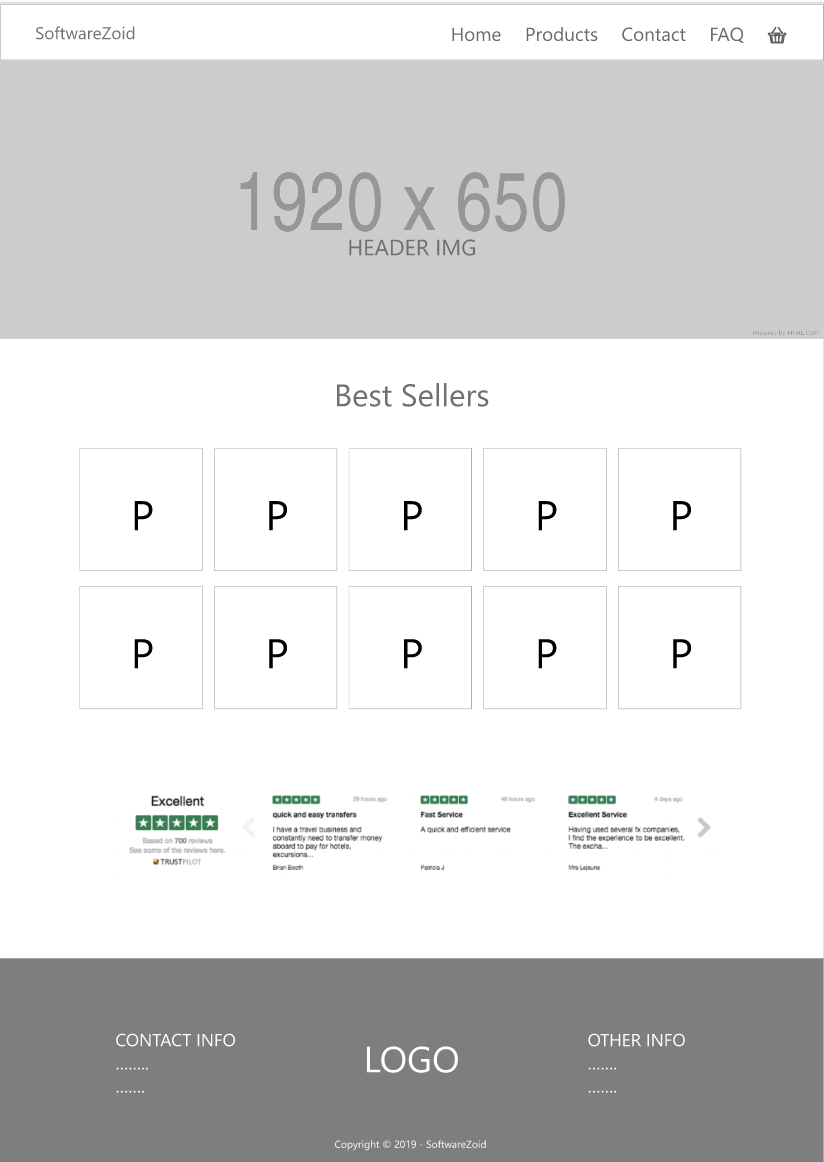
\includegraphics[height=17cm]{page1}
\end{center}
\noindent This page consists of 3 sections:
\begin{itemize}
  \item Header image: The width scales with the page, the height is fixed, though it doesn’t have to be “650”
  \item Best Sellers: Shows the best selling products, where P is the product with an image, title and price.
  \item Reviews: Must show 4 reviews per page in the slider. Contains stars, title, info and name.
\end{itemize}

\begin{center}
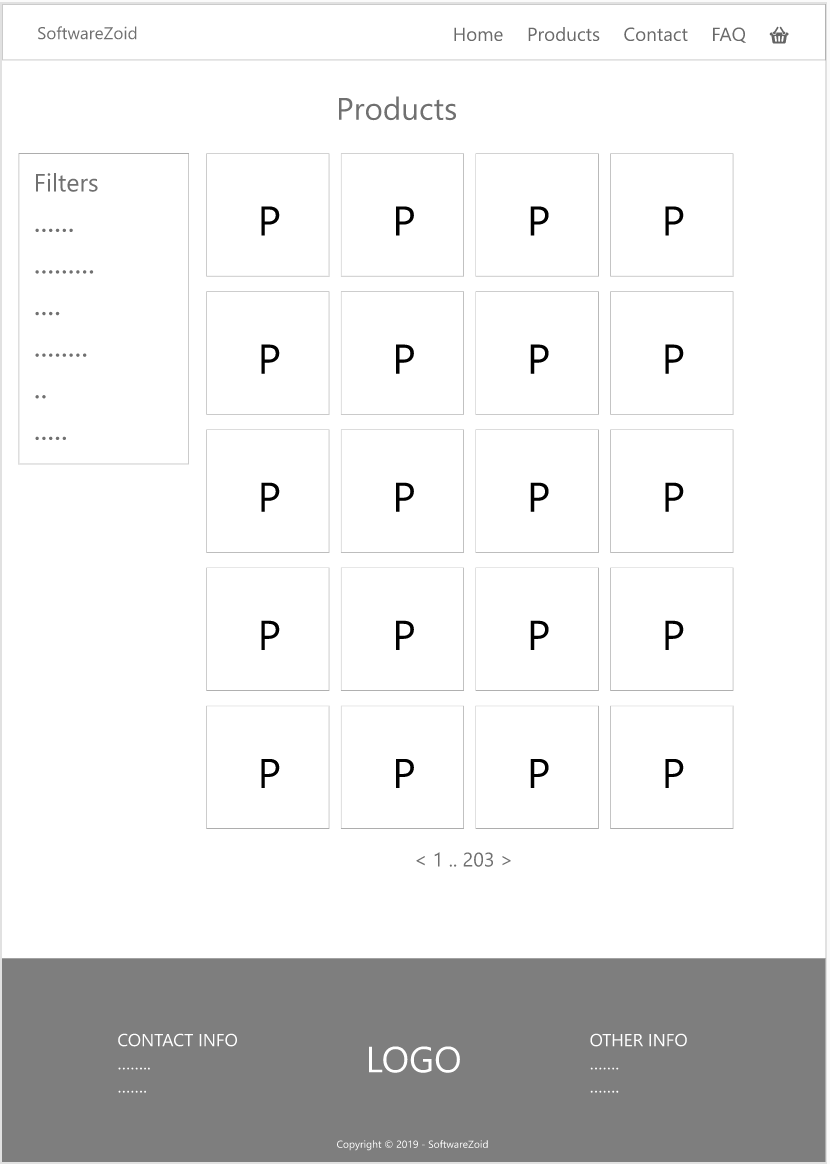
\includegraphics[height=17cm]{page2}
\end{center}
\noindent The products page, for each P(product) it should include an image, title and price. The filters (on the left side) includes a checkbox, slighter and a dropdownbox. The 3 components must be reusable. We also need pagination under each product.

\begin{center}
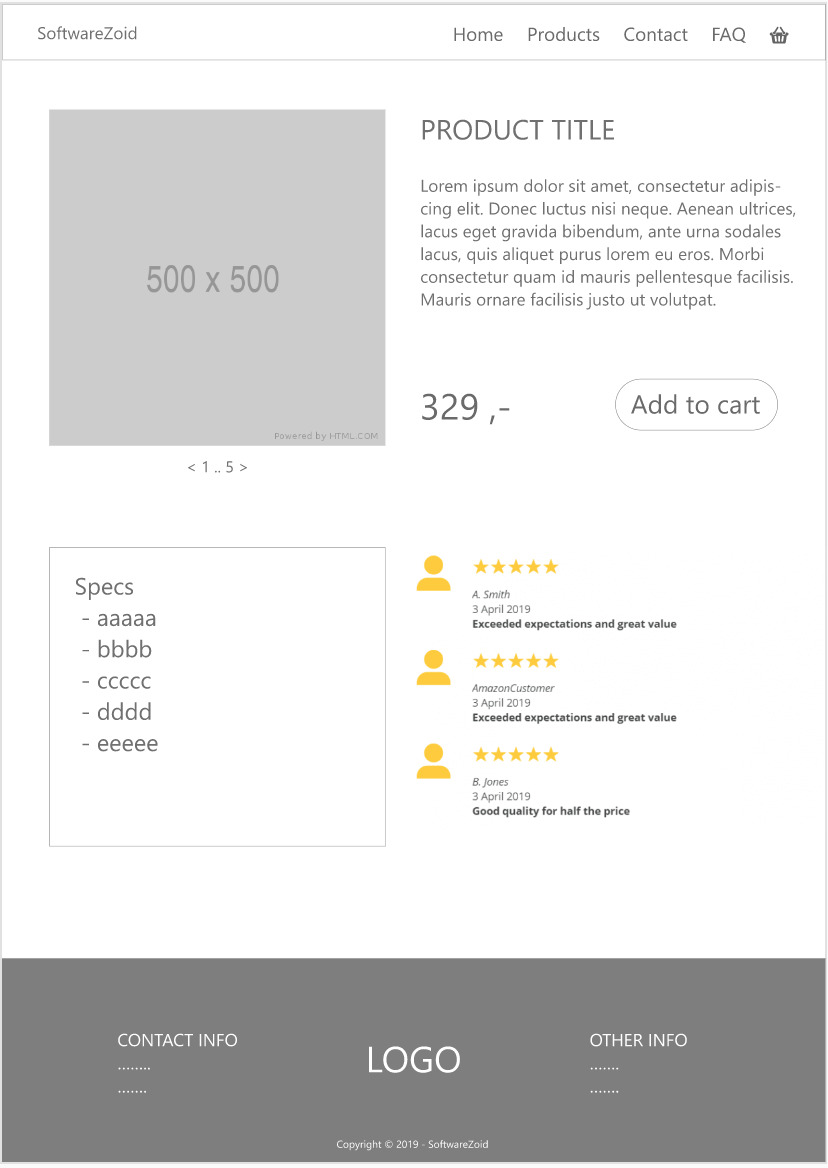
\includegraphics[height=17cm]{page3}
\end{center}
\noindent This page consists of images of the given product with pagination under it. The page includes a product title, a description of the product and a button. The specs must be made as a table of the most important information on the product. This page also includes reviews of the product which includes a rating, name, date and info.

\begin{center}
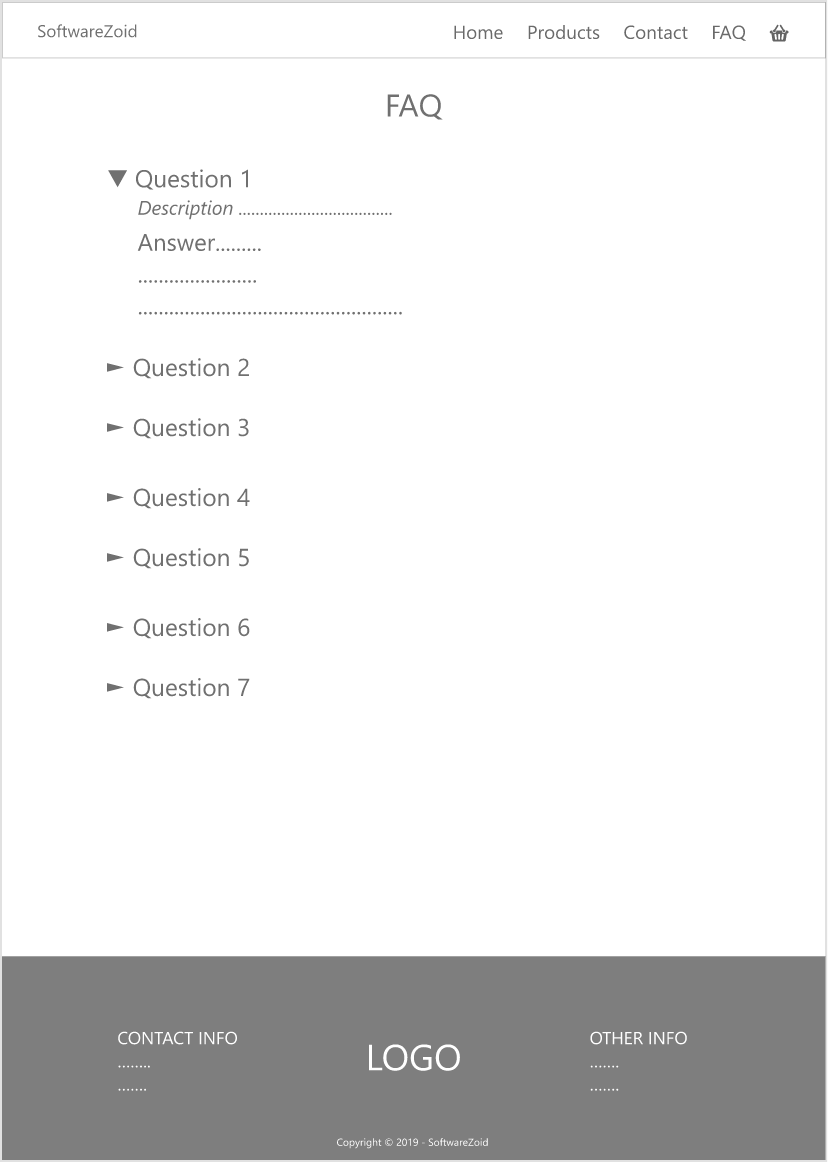
\includegraphics[height=17cm]{page4}
\end{center}
\noindent FAQ has 1 section
\begin{itemize}
  \item This section consists of several questions of which are dropdowns. The description and answer to the question is only shown when the question is clicked/opened.
\end{itemize}

\begin{center}
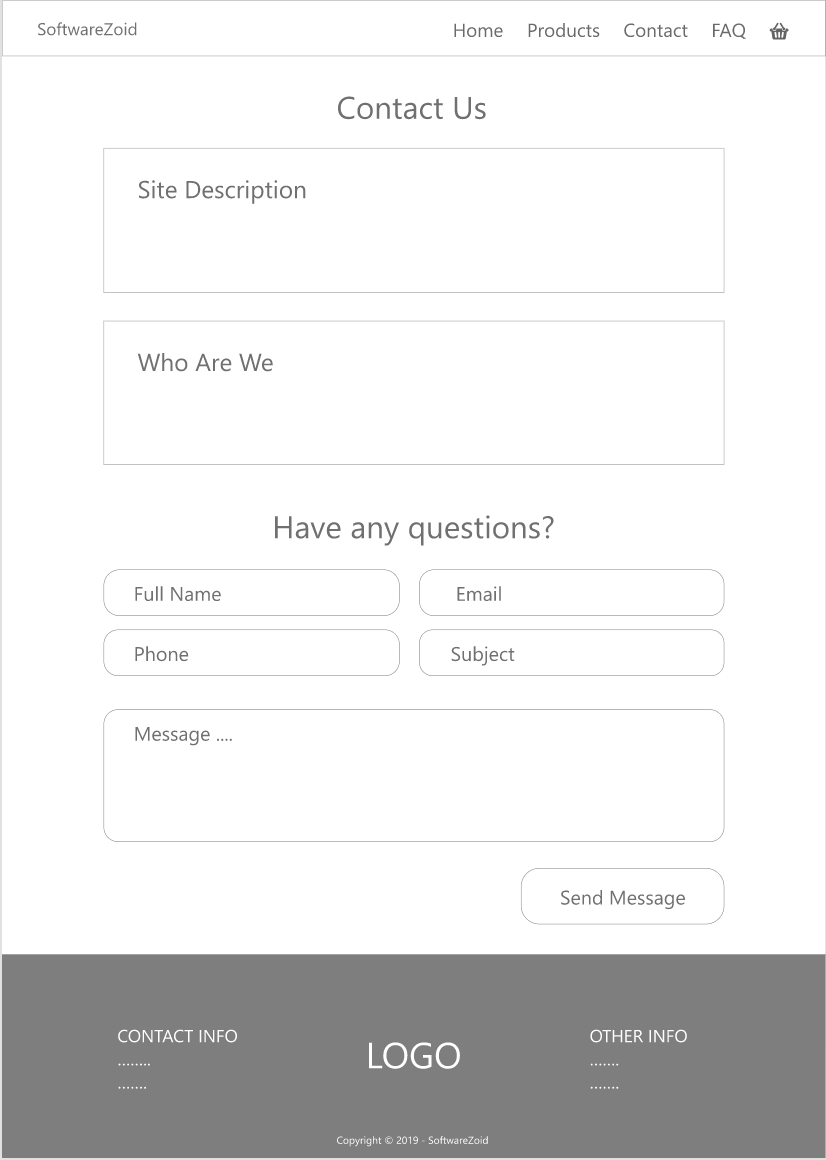
\includegraphics[height=17cm]{page5}
\end{center}
\noindent The contact page consist of 3 sections:
\begin{itemize}
  \item A site description and a “who are we”: Has to show a lot of text in a pretty and manageable way.
  \item Have any Questions: a form with these input fields: full name, email, phone, subject and message.
\end{itemize}

\begin{center}
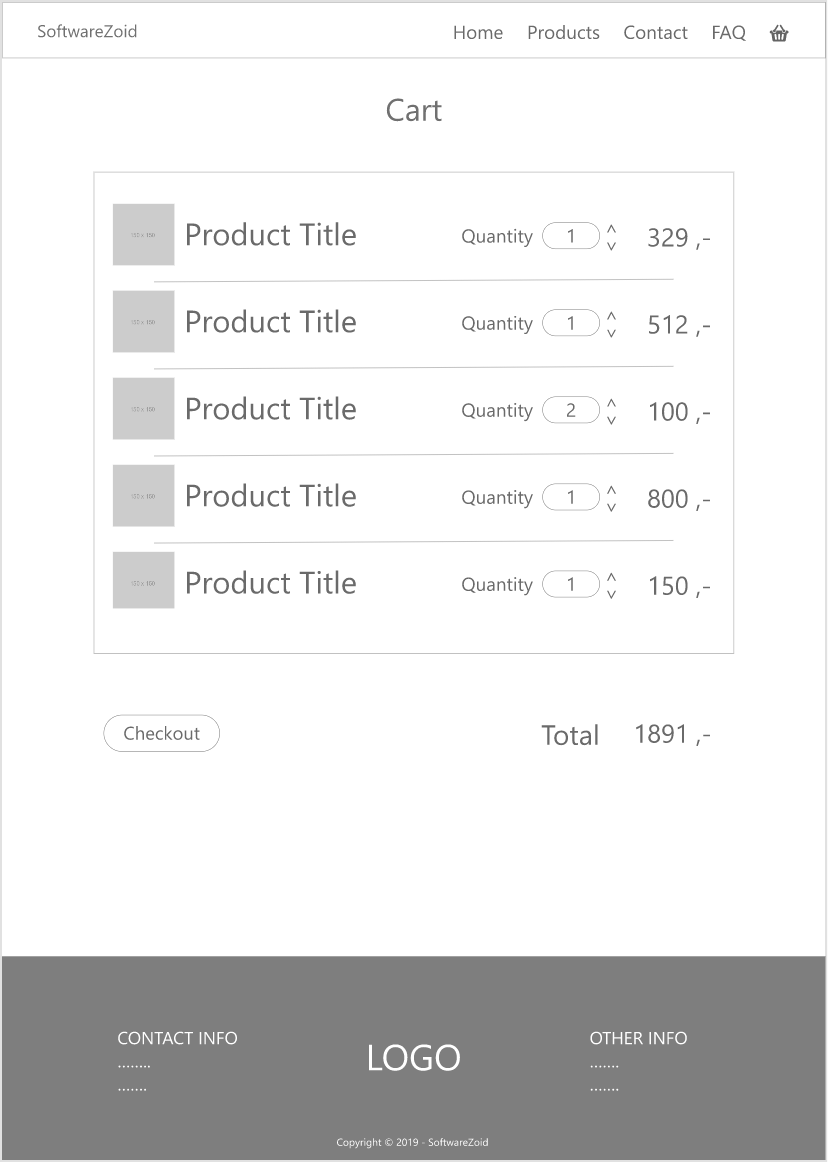
\includegraphics[height=17cm]{page6}
\end{center}
\noindent The cart page has a list of all the products that the customer has put in their basket, has to be presented in a table. In each table row there must be a product image, a product title, a display of quantity, and a price. Under the table there has to be a checkout button, alongside with a total price for all products in the basket.

\begin{center}
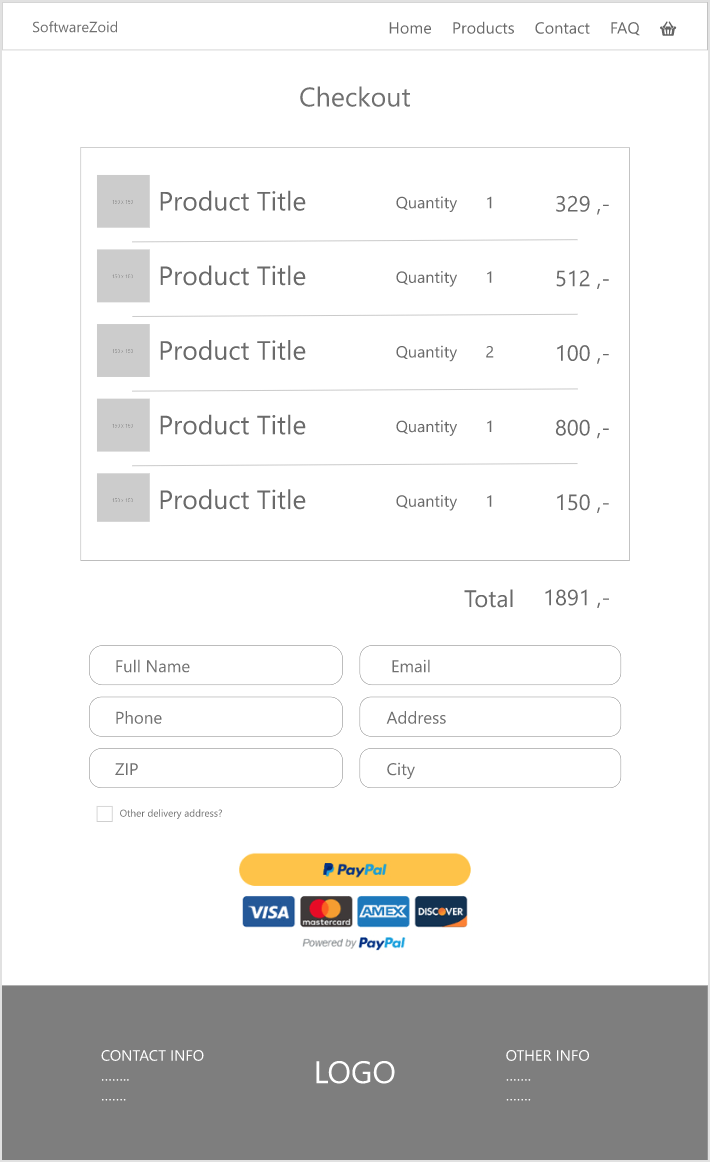
\includegraphics[height=17cm]{page7}
\end{center}
\noindent The checkout page will contain a list of the products that were put in cart, shown in a table. In each table row there has to be a product image, product title, quantity and product price. Under the table there has to be a display of the total price and a checkout form. The checkout form must contain following fields: full name, email, phone, address, zip and city, the form must also include a checkbox for alternative shipping address. Lastly a pay with paypal button.

\newpage
\section*{11.3 Bilag 3) Outsorce Korrespondance af webdesign}
\addcontentsline{toc}{section}{11.3 Bilag 3) Outsorce Korrespondance af webdesign}

\noindent\underline{Tuesday, November 12, 2019 – Andreas Vikke}\\
\noindent We're a team of backend developers that are working with a client that sells software and software packages.

\noindent We're looking for a frontend designer with a simplistic form of creativity, and likes the creative style of minimalism. The actual design of the frontend page(s) is not specified, you will be provided a sketch of how and where labels and buttons should be places, but we will gladly take input from you if you have better ideas.

\noindent We do although require that the code is documented to some degree with comments so that we can more smoothly integrate it with our backend. We also require that you as the designer can both understand, and write English.

\noindent The sketch is made in Adobe XD, and provided here there's a demo page:

\noindent https://xd.adobe.com/view/5da95fa7-c677-44d6-6430-3383f6cf8c37-2b98/ (Bilag 2)

\noindent (Attached is the 3 files: The Sketch in PDF and XD format, and a general description PDF of all the pages)

Est. Budget: \$200.00

Milestone 1: Basic Structure / design

Due: Friday, November 15, 2019

Amount in escrow: \$50.00 

\noindent\underline{Tuesday, November 12, 2019 – Andreas Vikke}\\
\noindent Hello Ahmed, I found your profile and previous work very well done, and I'm hoping you'll accept our offer. If you have any questions regarding the milestones or their meanings please do contact me.

\noindent\underline{Tuesday, November 12, 2019 – Ahmed Hassan}\\
\noindent Hello Andreas I will check the attached files now and get back to you

\noindent\underline{Tuesday, November 12, 2019 – Andreas Vikke}\\
\noindent Perfect, thank you.


\noindent\underline{Tuesday, November 12, 2019 – Ahmed Hassan}\\
\noindent Hello Andreas, I checked the files and I can start in anytime , thank you.

\noindent\underline{Tuesday, November 12, 2019 – Ahmed Hassan}\\
\noindent Ahmed Hassan accepted the offer

\noindent I will start now can I know if you use angular for front-end ?

\noindent also I will use scss is this good for you or you preferred css ?

\noindent\underline{Tuesday, November 12, 2019 – Andreas Vikke}\\
\noindent We use react for front end, not angular.

\noindent You can use scss, as long as you provide us with a css file afterwards

\noindent Both the scss and css file i mean :)

\noindent\underline{Tuesday, November 12, 2019 – Ahmed Hassan}\\
\noindent great, thank you.

\noindent\underline{Tuesday, November 12, 2019 – Andreas Vikke}\\
\noindent Looking forward to seeing what you make :)

\noindent\underline{Tuesday, November 12, 2019 – Ahmed Hassan}\\
\noindent I will do my best :)

\noindent\underline{Tuesday, November 14, 2019 – Andreas Vikke}\\
\noindent Hello Ahmed, do you have some basic structure and design you can show me as per the first milestone? :)

\noindent\underline{Tuesday, November 14, 2019 – Ahmed Hassan}\\
\noindent Hello Andreas, I will give you tonight the layout and home page, don’t worry :)


\noindent\underline{Tuesday, November 15, 2019 – Ahmed Hassan}\\
\noindent Ahmed Hassan requested payment for the milestone

\noindent this is the layout and home page also I create a global css buttons and selectors.

\noindent I added overview section, our team and contact us.I think Contact us is important to be in home page but if you want to delete any section I will.

\noindent please give me your feedback or changes If you want to change anything

Milestone 1: "Basic Structure / design"

Due: Friday, November 15, 2019

Amount: \$50.00

\noindent\underline{Tuesday, November 15, 2019 – Andreas Vikke}\\
\noindent Hello Ahmed, at first glance it looks great! my team is just reviewing it and coming with thoughts and changes, then i will send them and the money to you :)

\noindent\underline{Tuesday, November 15, 2019 – Ahmed Hassan}\\
\noindent Okay and also I will update small things to improve the homepage :)

\noindent\underline{Tuesday, November 15, 2019 – Andreas Vikke}\\
\noindent Sounds great! :)

\noindent\underline{Tuesday, November 15, 2019 – Andreas Vikke}\\
\noindent Hello Ahmed, everything seems very well. It seems like the buttons aren't really going to the right places though, FAQ goes to "best sellers", basket goes to contact us, contact us goes to a "about us" section. I'm assuming this is because the faq and cart page haven't been made yet? :)

\noindent We like the OPA style that you've made, although we don't need an about us section as a "our team" sort of thing.

\noindent I think it's a good idea with the contact section being on the home page, i haven't heard any comments from my team regarding this though, so we'll keep it like that for now :)

\noindent Now that the basic structure and design is in place, we're just missing some of the remaining pages (Specifik product page, FAQ, basket and checkout). As said you still have your artistic freedom over these pages as long as long as it has the requirements from the sketch (e.g. specific product has title, description, price and so on).

\noindent If you have any questions or uncertainties, don't hesitate to write me, I'll respond as quickly as possible.

\noindent Looking forward to what you produce :)

\noindent Andreas Vikke approved the milestone

Milestone 1: "Basic Structure / design"

Due: Friday, November 15, 2019

Amount paid: \$50.00

Amount: \$50.00

\noindent Andreas Vikke activated the milestone

Milestone 2: "Final Outcast/Evaluation"

Due: Sunday, November 17, 2019

Amount: \$50.00

\noindent\underline{Tuesday, November 15, 2019 – Andreas Vikke}\\
\noindent For the final Outcast we'd like that the specific single products get their own page, as well as faq, basket and checkout. :)

\noindent\underline{Tuesday, November 16, 2019 – Ahmed Hassan}\\
\noindent Don’t worry in the final outcast everything will be like you want :)

\noindent\underline{Tuesday, November 16, 2019 – Andreas Vikke}\\
\noindent Perfect! :)
\newpage
\noindent\underline{Tuesday, November 16, 2019 – Ahmed Hassan}\\
\noindent Ahmed Hassan requested payment for the milestone

\noindent please check the whole website design and I still have some work with it

Milestone 2: "Final Outcast/Evaluation"

Due: Sunday, November 17, 2019

Amount: \$50.00

\noindent\underline{Tuesday, November 16, 2019 – Andreas Vikke}\\
\noindent Hello Ahmed, very impressive! :)

\noindent We do have a few pointers though:

\noindent I can see you haven't quite finished the contact page, and that the navlink contact currently goes to whatever page it is currently on, that of course just needs fixing and I'm assuming that this is what you mean with you still have some work to do :)

\noindent On the basket page i can see that there's a payment option, we only want that in the checkout page.

\noindent On the product page, the filter tab is responsive with the body and the body shrinks according to the filter, but the footer does not, we'd like that it does as well.

\noindent I can see we are also missing the page when you click on "more details" on a product. i can see it's there, it's just not linked from what i can get. :)

\noindent I haven't been able to check yet wether or not it looks nice on mobile, but this is also important to us, that the website can adapt to this.

\noindent So just the last bits and mobile friendly and we're about there! We're very happy with what you've provided so far, looks very nice!

\noindent Andreas Vikke approved the milestone

Milestone 2: "Final Outcast/Evaluation"

Due: Sunday, November 17, 2019

Amount paid: \$50.00

Amount: \$50.00
\newpage
\noindent Andreas Vikke activated the milestone

Milestone 3: "Final Product"

Due: Tuesday, November 19, 2019

Amount: \$100.00


\noindent\underline{Tuesday, November 19, 2019 – Andreas Vikke}\\
\noindent Did you see and understand my message Ahmed? :)

\noindent\underline{Tuesday, November 19, 2019 – Ahmed Hassan}\\
\noindent Yes I am working now to give you final design :)

\noindent\underline{Tuesday, November 19, 2019 – Andreas Vikke}\\
\noindent Perfect! :)

\noindent\underline{Tuesday, November 19, 2019 – Ahmed Hassan}\\
\noindent Ahmed Hassan requested payment for the milestone

\noindent Milestone 3: "Final Product"

Due: Tuesday, November 19, 2019

Amount: \$100.00    

\noindent this the final version please check it and if you face any problem send to me anytime also if you face any problem in my work after closing the contract I will fix it for free :)


\noindent\underline{Tuesday, November 19, 2019 – Andreas Vikke}\\
\noindent Perfect, we're just going to look it through and I'll come back to you, at first glance here it looks amazing :)

\noindent\underline{Tuesday, November 19, 2019 – Andreas Vikke}\\
\noindent I've sent it off to the rest of my team, and awaiting to hear some response and feedback from them, but i noticed some small details I'd liked fixed :)

\noindent When in basket, continue shopping doesn't go to products.

\noindent Also in basket, the home link doesn't respond when clicked (can't go from basket to home).

\noindent When on products page, notice how it's not the same logo in the cart as in all other pages, we'd like that the logo for the cart is consistent throughout the pages.

\noindent That's what i just noticed quickly looking through it, I'll send the feedback if i get any later today, and if i don't get anything I'll just send you the money :)

\noindent\underline{Tuesday, November 19, 2019 – Ahmed Hassan}\\
\noindent okay bro, I fixed the issues that you noticed :)

\noindent\underline{Tuesday, November 19, 2019 – Andreas Vikke}\\
\noindent It looks good, some things went missing and/or misaligned though

\noindent Filter icon gone and misalignments in the cart

\noindent\underline{Tuesday, November 19, 2019 – Ahmed Hassan}\\
\noindent oh, sorry :D

\noindent\underline{Tuesday, November 19, 2019 – Andreas Vikke}\\
\noindent Perfect, thanks ^^ haven't heard back from my team yet, but expecting some feedback soon! :)

\noindent\underline{Tuesday, November 19, 2019 – Andreas Vikke}\\
\noindent So what seems to be the last feedback is that we'd like a "back" button from product details to products, do you think you could do that quickly? :)

\noindent\underline{Tuesday, November 19, 2019 – Ahmed Hassan}\\
\noindent I added it :)

\noindent\underline{Tuesday, November 19, 2019 – Andreas Vikke}\\
\noindent Perfect, thank you very much ^^ My team doesn't seem to have any more feedback, so i thank you for your help! :)

\noindent Andreas Vikke approved the milestone

Milestone 3: "Final Product"

Due: Tuesday, November 19, 2019

Amount paid: \$100.00

Amount: \$100.00

\noindent\underline{Tuesday, November 19, 2019 – Andreas Vikke}\\
\noindent Andreas Vikke ended the contract

\noindent\underline{Tuesday, November 19, 2019 – Ahmed Hassan}\\
\noindent thanks you very much , I am here anytime if you need any help :) I hope you give me a good feedback :)

\noindent\underline{Tuesday, November 19, 2019 – Andreas Vikke}\\
\noindent Thank you very much :) and I've given you 5 stars a long with a good review text :D

\noindent\underline{Tuesday, November 19, 2019 – Ahmed Hassan}\\
\noindent thank you :)


\newpage
\section*{11.4 Bilag 4) Outsorce Korrespondance af 404 side}
\addcontentsline{toc}{section}{11.4 Bilag 4) Outsorce Korrespondance af 404 side}

\noindent\underline{3. Dec. - William Huusfeldt}
\begin{enumerate}
\item \textbf{Your existing website link to get the feel of your website.}
The website that we're building is linked below.
softwarezoid.surge.sh
\item \textbf{Any special requirements for your design}
Be as creative as you like, however, we'd like it that the page reflects that we're dealing with software sales.
\end{enumerate}

\noindent\underline{3. Dec. - Mizanur}\\
\noindent Hello, thanks very much for your order. Unfortunately, I am out of my workplace until tomorrow. Will it be possible for you to increase the deadline by 2 days? I promise to get back to work as soon as I return to my workplace. Thanks.

\noindent\underline{3. Dec. - William}\\
\noindent Hi again, That's quite alright.

\noindent\underline{3. Dec. - Mizanur}\\
\noindent Thank you very much. I really appreciate it.

\noindent\underline{3. Dec. - Mizanur}\\
\noindent to clarify, you need a 404 page design both in Photoshop and HTML and CSS? 
\noindent Did I get it right?

\noindent\underline{3. Dec. - William}\\
\noindent No problem :)
\noindent HTML and CSS is top priority and actually mainly what we're looking for, and yes, it's a 404 page we'd like to get.

\noindent\underline{3. Dec. - Mizanur}\\
\noindent Thank you for your reply. I will get back to you as soon as I can. In the meantime, I am sending you a request to extend the deadline by two days. Please accept. Thanks.

\noindent -- Deadline rykkes 2 dage til d. 7. Dec.

\noindent\underline{6. Dec. - Mizanur}\\
\noindent Hello, I have made designed the page. I have followed the design style, color and font combination of your current website. I hope you will like it. Please have a look and give your feedback. Thanks.

\noindent\underline{6. Dec. - William}\\
\noindent Perfect, thank you!

\noindent\underline{6. Dec. - Mizanur}\\
\noindent Hi willhuusfeldt,
\noindent Thanks again for your order! Your delivery is enclosed. You will find the source files in the zip format attached here. If there are any problems, please let me know. I'll get back to you as soon as I can.

\noindent If you need anything to change in the design please message me. Don't forget to appreciate me in the comments.

\noindent Thanks again and have a great day! :)

\noindent Mdmizanur3950

\noindent -- Godkendt


\newpage
\section*{11.5 Bilag 5) Outsorce Korrespondance af Favicon}
\addcontentsline{toc}{section}{11.5 Bilag 5) Outsorce Korrespondance af Favicon}


\noindent\underline{4. Dec. - William Huusfeldt:}\\
\noindent This is our website softwarezoid.surge.sh

\noindent We don't have a logo per se, so take inspiration from the site and make something that you think fits the site.

\noindent Regards, William

\noindent\underline{4. Dec. - Pro\_Graphics\_4U:}\\
\noindent Hey willhuusfeldt, please see the attached files.

\noindent I added you even bonus (source file)

\noindent Before leaving feedback, please let me know if you have ANY issues with your files and I'll do everything in my power to correct it for you at no additional charge.

\noindent If you like it, I would sincerely appreciate a good and honest review.

\noindent I want you to be 100\% satisfied with my work, otherwise, I insist that you ask me for a full refund. No hard feelings.

\noindent Ps. Do you have any more work to do? Or something you are struggling with?

\noindent Thank you, Regards Cris

\noindent -- Godkendt

\newpage
\section*{11.22 Bilag 22}
\addcontentsline{toc}{section}{11.22 Bilag 22}
Første Sprint\\
\textbf{\#12 Som sælger, vil jeg gerne generer styklister for en carport med faste mål uden hældning og uden skur.}\\
Størrelse: XXLarge\\
Acceptance kriterium: Skal beregne 100\% korrekt for mål uden hældning og skur.\\
Subtasks:
\begin{itemize}
\item \#18 Beregn stykliste for taget (12 timer).
\item \#19 Beregn stykliste for mål (12 timer).
\item \#20 Indsæt data i List (1 time).
\item \#28 Opret database/Opret lager tabel (1 time).
\item \#30 Indsæt dummy data (2 timer).
\item \#31 Datamappers (2 timer).
\item \#32 Database Connector (2 timer).
\item \#37 Print stykliste til terminal (1 time).
\end{itemize}
\leavevmode

\end{document}

